%!TEX root = thesis.tex 

\chapter{Use Cases} \label{cha:Use Cases}
	\paragraph{}
	In Chapter \ref{cha:An Alternative Approach} we detailed the requirements and design of our linking solution. In Chapter \ref{cha:The Tool} we discussed the technical details of our first prototype. During these past few chapters we have claimed that our tool addresses many of the inherit problems of the current HTML standard with respect to hyperlinking. We also claimed to solve many of the issues of previously developed tools that  attempted to enhance the web's linking techniques.
	\paragraph{}
	In this chapter we would like to validate our claims. The time restriction of this thesis did not allow us to evaluate our solution by means of user trails. So instead we would like to validate our solution by presenting a couple of use cases. By walking through the process of authoring hyperlinks, navigating and rating existing links and searching the database of metadata for information.
	\paragraph{}
	As the reader most likely has had experience with authoring hyperlinks in standard HTML, and navigating the web using conventional browsers, one can compare the presented process with other tools as we walk through the scenario.
	\paragraph{}
	We hope to demonstrate that our tool indeed improves upon the standard HTML way of linking, as well as the approaches of many other existing tools.
	\paragraph{}
	We are however quite aware that our solution is not perfect, and will fall short on certain aspects. To demonstrate where the tool falters we will also present a couple of use cases that will not yield desirable results.

\section{Scenarios} \label{sec:Scenarios}
	\paragraph{}
	First of all we need a couple of scenarios that we will use to demonstrate different aspects of the tool. Using real concrete scenarios will help us define the needs and expectations of the user. So instead of using hypothetical scenarios we will use some that the reader can relate to.
	\subsection{Authoring} \label{sub:Authoring}
		\subsubsection*{Adding a Comment} \label{sub:Adding a Comment}
			\paragraph{}
			A user is reading an article about rendezvous manoeuvres between spacecrafts in orbit. But he notices that the content has no documentation about the mathematics behind the manoeuvres and is wondering where he can find this information. Instead of trying to find this information himself he wants to post a comment on this section asking for more information on this.
			\paragraph{}
			This scenario describes the basic need to add data to already existing data. There is no notion of hyperlinking yet. The user just wants to attach one resource (in this case a question in the form of an annotation) to another resource (in this case the web page). This basic example serves as a demonstration of how to author the most simple metadata.
			\paragraph{}
			So here are the steps the user will take to accomplish his goal. First he will select the relevant context on the web page. When his selection is complete he will click the \dquote{Add Comment} Button from the tool bar. The tool will open a pop-up window in which the user can fill in the rest of his data. The user will write his question in the text box, and add the \dquote{Question} tag to his comment. With all information in place the user submits the form to the server.
			\begin{figure}[h]
				\centering
				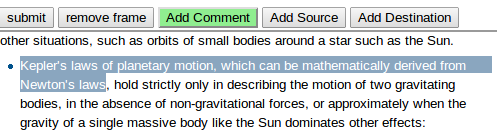
\includegraphics[width=\textwidth*4/5]{usecase/addComment.png}
				\caption{Making a selection}
			\end{figure}
			\begin{figure}[h]
				\centering
				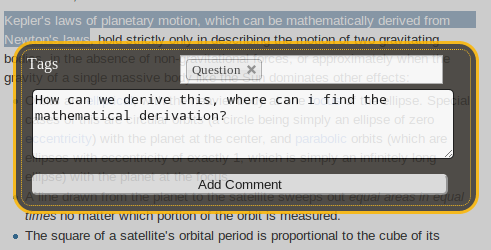
\includegraphics[width=\textwidth*4/5]{usecase/addCommentForm.png}
				\caption{Posting a comment}
			\end{figure}
			\paragraph{}
			This process of adding annotations or questions to certain parts of a web page feel very intuitive. Selecting a part of text, and writing a side note in the form fit the metaphor of highlighting a paragraph in a textbook and writing a note in the margin.
		\subsubsection*{Adding a Hyperlink} \label{sub:Adding a Hyperlink}
			\paragraph{}
			In this scenario the user does not want to ask the question about where he can find the mathematical explanation. Instead he already knows a reliable source where these calculations are explained very well. Therefore instead of adding a comment, or a note it would be much easier for the user if he could just create a hyperlink between the two documents.
			\paragraph{}
			To create the hyperlink the user needs to open a second frame by clicking the \dquote{Add Frame} button. This will split the window in two frames. Each of the frames will be able to load a different web page. In the first frame the user surfs to the web page he wanted to add the link to. In the second frame he will navigate to the web page containing the additional information that he wants the link to point to.
			\paragraph{}
			Having both these web pages open the users creates a selection on the first web page, the same way he would have done if he wanted to add a comment to the pages, as described in the previous scenario. In the second frame he will create a selection as well. This time the selection is the context of the extra information that was relevant to the selection in the first frame.
			\begin{figure}[H]
				\centering
				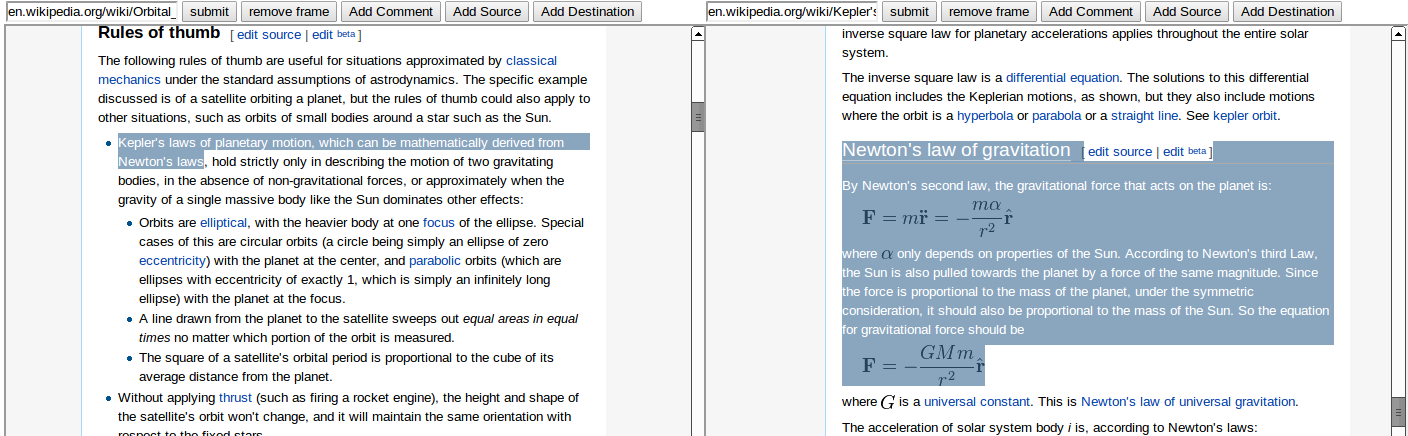
\includegraphics[width=\textwidth]{usecase/addLink.png}
				\caption{Adding a second frame with its own selection}
			\end{figure}
			\paragraph{}
			With both selections in place the user clicks the \dquote{Create Link} button in the tool bar. Clicking this button will open another pop-up window. Here the user will be presented with the option to add tags to his hyperlink and because these tags significantly help other users to find the required information the user will fill in these tags as best as possible tagging the link with \dquote{Rendezvous Manoeuvre, Mathematics, Formula}.
			\begin{figure}[h]
				\centering
				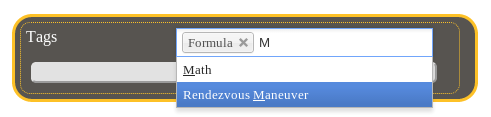
\includegraphics[width=\textwidth*4/5]{usecase/addLinkForm.png}
				\caption{Adding tags to hyperlink when the system guesses the roles}
			\end{figure}
		\subsubsection*{Multi Destination Hyperlink} \label{sub:Multi Destination Hyperlink}
			\paragraph{}
			In the previous scenario the user only linked to a single web page. Because he only had two frames open, each containing a web page the tool assumed that by clicking the \dquote{Create Link} button the user meant to create a link with one source (the left frame), and one destination (the right frame). This assumption is the intuitive approach when a user adds two documents together and therefore using \dquote{Convention Over Configuration} will speed up the process of creating these simple links.
			\paragraph{}
			In this scenario however, the link to be constructed is no longer a simple one. The user in this scenario knows about an interesting web page that describes the mathematics behind the rendezvous manoeuvre. But he also knows about a scientific paper in PDF format that explains the mathematics in far greater detail. Off course having to create two separate links for these two resources is a lot of work. So the user wants to link both of these resources to the web page in one hyperlink.
			\paragraph{}
			The process of doing so is fairly similar to the previous scenario. The difference is that the tool can no longer easily guess what frames contain the destinations, and which frame contains the source of the link. So the user will do as follows. He opens 2 additional frames in one of these frames he will navigate to the other web page he wanted to link to and in the second frame he will navigate to the PDF document. A third frame, that was already open, contains the original web page on which the link needs to be constructed.
			\paragraph{}
			With three frames open the user proceeds by specifying which frame serves what purpose. The user will click on the \dquote{Source} check mark above the third frame, specifying that the selection in this frame will be used as a source. The two other frames will be marked as destinations in the same way. With these specifications in place the user proceeds to click on the \dquote{Create Link} button and is again prompted with a similar pop-up window.
			\paragraph{}
			In this pop-up window the user can again specify the tags to describe the links. And he will do so in the same way as the previous scenario. But there is a difference here. Each destination of the link can have its own characteristics so tags can be added per destination as well. The user will do so by additionally specifying that the second destination is in fact a PDF document by adding the tag \dquote{PDF}. The three other tags are general shared tags between both destinations, while the specific \dquote{PDF} tag only applies to the second one.
			\begin{figure}[h]
				\centering
				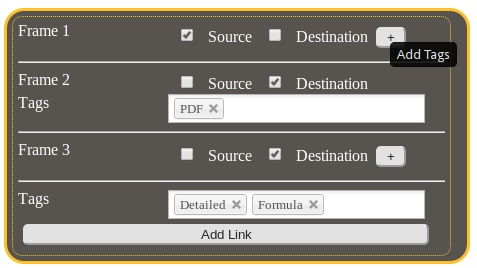
\includegraphics[width=\textwidth*4/5]{usecase/addMultiLinkForm.png}
				\caption{Manually specifying roles for selectors}
			\end{figure}
			\paragraph{}
			Any combination of many sources and many destinations can be constructed this way. The user only needs to add more selections in new frames and select the role for each of these frames.
		\subsubsection*{Multi Source On a Single Page} \label{sub:Multi Source On a Single Page}
			\paragraph{}
			In this scenario the user wants to add refer to a web page again describing the details about the mathematics behind a rendezvous manoeuvre. But instead of linking to this page from a single paragraph in on the web page he wants to link to the same web page in several separate locations in the text. A few spread out paragraphs may mention the manoeuvre but instead of providing the hyperlink only where it is mentioned first he wants to create a hyperlink on each mention of the manoeuvre.
			\paragraph{}
			The user could use the same approach as described with the previous scenario, but this would require him to open several frames displaying the same document for the sole purpose of creating several selections. This is off course cumbersome.
			\paragraph{}
			Instead the user may open two frames, the first containing the source document and the second frame containing the destination of the hyperlink. The user will then create a first selection on the first frame which represent one of the sources of the hyperlink. He will then press the \dquote{Add Source} button from the tool bar. This will temporarily save his selection and mark this selection as a source for the next creation of a hyperlink. Pressing this button will also remove the selection on that frame leaving room for a new selection.
			\begin{figure}[h]
				\centering
				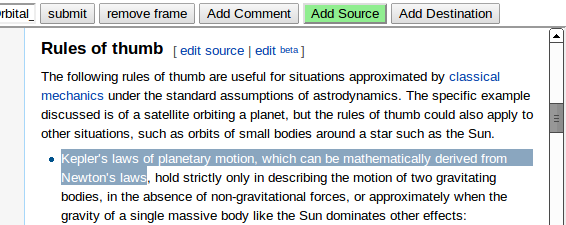
\includegraphics[width=\textwidth*4/5]{usecase/addSource.png}
			\end{figure}
			\begin{figure}[h]
				\centering
				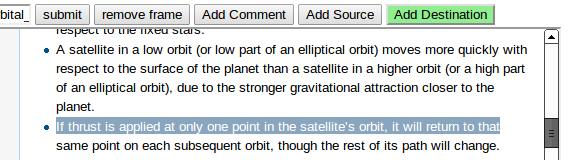
\includegraphics[width=\textwidth*4/5]{usecase/addDestination.png}
				\caption{Specify a role for an active selection}
			\end{figure}
			\paragraph{}
			After the user has selected all the locations in this document that he wants to use as a source he can do the same with any of the other frames. Marking each selection as a source or destination. When the user is done creating his selections and adding them to the appropriate roles he clicks the \dquote{Create Link} button and is presented with a familiar pop-up window prompting for more information. When the user is finished filling in the tags he will submit the form, creating the hyperlink for future users.
			\begin{figure}[h]
				\centering
				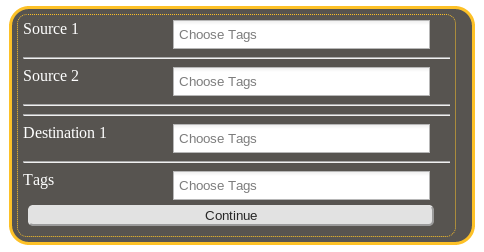
\includegraphics[width=\textwidth*4/5]{usecase/addMultiLinkManualForm.png}
				\caption{Adding tags to respective sources and destinations}
			\end{figure}
	\subsection{Navigation} \label{sub:Navigation}
	\subsubsection*{Following a Hyperlink} \label{sub:Following a Hyperlink}
		\paragraph{}
		In this scenario the user is reading the paragraph about the rendezvous manoeuvres and he wants to find more information about this topic. In order to find out if the community has already provided some hyperlinks he highlights the relevant context. This selection will update the graph view at the bottom of the screen which will now represent the metadata that is available for the selected context.
		\begin{figure}[h]
			\centering
			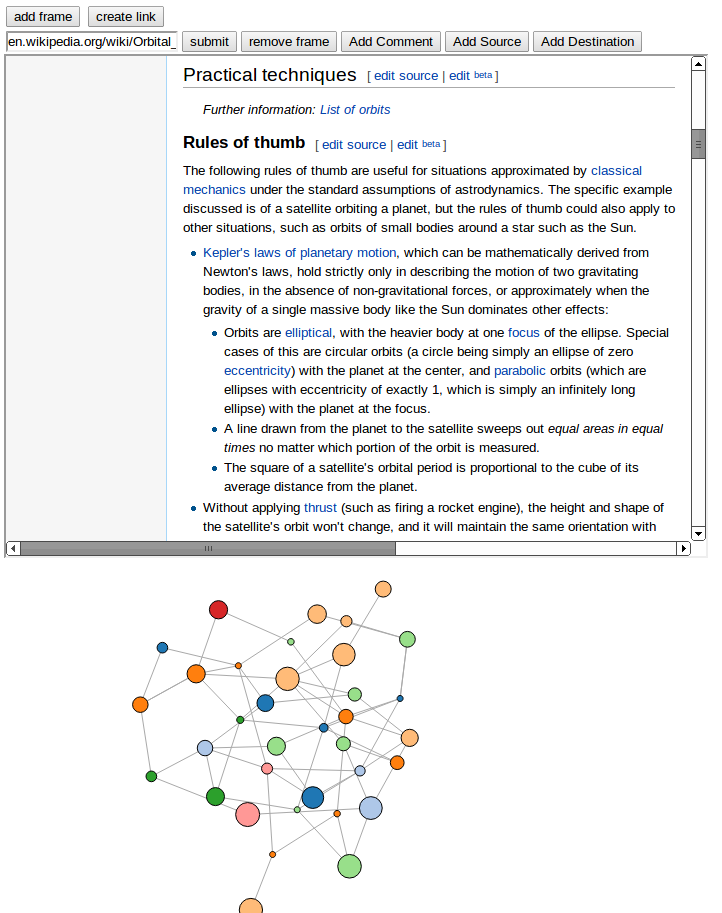
\includegraphics[width=\textwidth*4/5]{usecase/frameWithGraph.png}
			\caption{Graph and frame with no selections}
		\end{figure}
		\paragraph{}
		In this graph the user can now find all the outgoing links in his selection. Since previously other users have already added a couple of links to a web page, as well as a PDF file the user will notice this based on the colour codes of the nodes. The user is interested in the web page, so he clicks on the associated node in the graph and the tool redirects him to the appropriate web page.
		\begin{figure}[h]
			\centering
			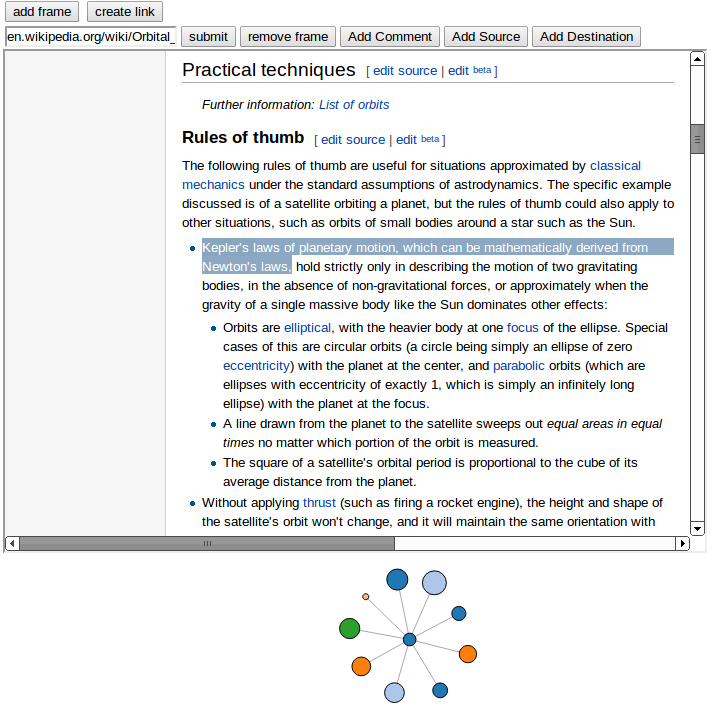
\includegraphics[width=\textwidth*4/5]{usecase/frameWithGraphSelected.png}
			\caption{Graph after making a selection}
		\end{figure}
	\subsubsection*{Searching Information} \label{ssub:Searching Information}
		\paragraph{}
		The user is faced with the same issue as the last scenario, but when he highlights the paragraph the resulting graph contains to many nodes to easily find the result he is looking for. The user is only interested in extra information about in the form of a PDF file. He also wants to find the exact mathematical formula instead of a long textual explanation about the manoeuvre. To find the intended result more quickly the users clicks in the search text field above the graph view and starts to add keywords to direct his search. The user first types the tag \dquote{PDF} but this renders far to many results to search through. Narrowing his search he will add the keyword \dquote{Formula} to the search query. Fortunately a hyperlink was added by a different user in the community containing both these tags and it is easy enough to find the requested result in the graph. Clicking on the associated node redirects the user to the requested PDF file
		\begin{figure}[h]
			\centering
			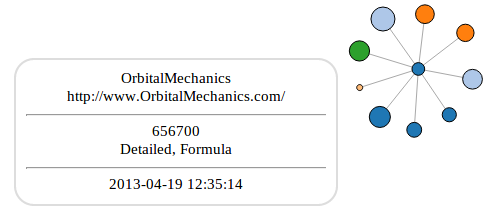
\includegraphics[width=\textwidth*4/5]{usecase/metadataGraph.png}
			\caption{Metadata on graph nodes}
		\end{figure}
	\subsection{Contribution} \label{sub:Contribution}
	\subsubsection*{Down Voting Existing Hyperlink} \label{sub:Down Voting Existing Hyperlink}
		\paragraph{}
		A user is reading the article and notices that there are two hyperlinks that point to the same resource. One of the two hyperlinks only points to a web page, while the second hyperlink points to the same web page, but also contains a PDF file as a second destination. When the user studies the extra metadata on both of the links, he notices that the tags and location of the first link are the same as the second one but the second hyperlink contains a better description as well. In short the user finds that the first hyperlink has been made obsolete by the second one. Seeing this the user wants to clear the web page of this redundant data for future users.
		\paragraph{}
		Down voting the link will help lower the popularity of the first hyperlink. Doing this will cause the redundant hyperlink to be hidden from other users. If other users will do the same eventually the obsolete metadata will be entirely removed from the web page, cleaning up the final result.
		\paragraph{}
		In order to do so the user right clicks on the node associated with the hyperlink. This will open a context menu on the node containing both the option to up or down vote the clicked hyperlink. The user then clicks on the \dquote{Down Vote} option. Doing this will send a request notifying the server of the user's contribution.
\section{Failing Scenarios} \label{sec:Failing Scenarios}
	\subsection{Blank Page} \label{sub:Blank Page}
		\paragraph{}
		In this scenario the user wants to add a simple annotation to a web page just as we described in the first scenario in the previous section. In order to do so the user opens a frame and enters the required URL in the appropriate field. But when the user submits the form nothing happens. The page stays on a black page.
		\paragraph{}
		This issue arises when a server disallows a web page to be served within a frame. The browser will notice that the \dquote{X-Frame-Option} is set in the header of the web page and will subsequently stop rendering the requested page.
		\paragraph{}
		Many large companies will not allow their website to be rendered within a frame. Companies such as Google, Facebook, Twitter, Microsoft, LinkedIn and many more will have this option set. This means that at the current state of the tool, many large and popular websites will not be able to be rendered by the tool.
	\subsection{Frame Killers} \label{sub:Frame Killers}
		\paragraph{}
		A similar situation occurs when a user wants to navigate the tool to MSN.com, Windows' live messenger website. Doing so will not yield a black page, but will in fact navigate the browser to the web page, instead of only the frame it was supposed to be loaded in. These website are running a script that, when loaded, checks whether or not the page was loaded in a frame. In the case of our tool this check will detect this and point the browser to the website instead of the frame. These frame killers, as they are called, will refresh the page which leads to a removal of the tool bars our tool provided. Therefore on these type of websites the users will not be able to add hyperlinks or comments.
	\subsection{Dynamic Pages} \label{sub:Result Mismatech}
		\paragraph{}
		In this example the user wants to add a link to a particular paragraph in an interesting blog posts. He will again select the source in the first frame, and the destination in the second frame, containing the blog. Clicking the \dquote{Create Link} button will finish the process and everything is in order. Users visiting the page will see the link, and following the link will direct them to the intended blog post.
		\paragraph{}
		However, a couple days later a users tries to follow the hyperlink and is redirected to the blog website. But the posts the user sees are not relevant to the context in which the link appeared. And in fact he can not see the destination of the link at all.
		\paragraph{}
		This effect is because of the way blog websites usually work. When the blogger adds a new post to his website the newest item will appear at the top, pushing all older items down. When to many items are on the front page the rest of the posts are paginated and require the reader to click on a link to see them. This behaviour is fairly standard but it poses a problem for the tool.
		\paragraph{}
		When a hyperlink is created the metadata for this link contains pointers to different resources, the sources of the hyperlink and the destinations. These resources can be PDF files, websites, video or audio files, and many more different types of media. In this case both the source and destination of the hyperlink are websites. The identifier of this resource is defined by its URL. So when the user links to the blog website he will create a pointer that points to a specific location in the resource that is identified by the specified URL. Lets say the destination of the hyperlink was a sentence in the first post of the website \dquote{www.blog.com}.
		\paragraph{}
		So on creation the hyperlink will work fine and point to the first post on the web page which, at the time, contained relevant information. After a while the owner of the blog will post new articles which will most likely not be related to the link's intended topic. Because of the restructuring of the web page the destination pointer of the hyperlink will no longer be valid. This will mislead or confuse visitors following the hyperlinks.
		\paragraph{}
		In Section \ref{sub:Workarounds} \nameref{sub:Workarounds} we already discussed some methods of helping with this problem but they are not infallible and the scenario we just described can still take place.
%	\subsection{Delayed Content} \label{sub:Delayed Content}
	
\section{Conclusion} \label{sec:Conclusion}
	\paragraph{}
	In this chapter, we have demonstrated some of the usages of our tool by means of some simple scenarios. As one can see many of the features are intuitive and simple to use providing an easy way of creating advanced links between different media. The functionality demonstrated by these simple examples represent only the beginning of the potential of the tool. When more visualisations are designed more features will be available for the user resulting in a richer user experience.
	\paragraph{}
	It is also important to note that many of the failing examples stem from restrictions in the current web standards. Security issues that plagued the web have resulted in a strict security protocol which dampens a lot of possibilities. And creating a more persistent way of selecting a part of a document will result in more robust linking overall.
